\documentclass[handout]{beamer}
%==============================================================
% Common Beamer Preamble for Course Lectures: Training and Scaling Language Models
%==============================================================

\usepackage[utf8]{inputenc}
\usepackage[T1]{fontenc}
\usepackage{hyperref}
\usepackage{amsmath,amssymb,xcolor,multicol,booktabs,colortbl}
\usepackage{graphicx,listings}
\renewcommand{\figurename}{Figure.}
\renewcommand{\tablename}{Table.}

% ---- TikZ Libraries ----
\usepackage{tikz}
\usetikzlibrary{positioning,arrows.meta,shapes.geometric,calc,fit,backgrounds,decorations.pathreplacing}

% ---- Presentation defaults ----
\setbeamertemplate{navigation symbols}{}
\setbeamersize{text margin left=0.55cm,text margin right=0.55cm}
\setbeamerfont{title}{size=\LARGE,series=\bfseries}
\setbeamerfont{subtitle}{size=\large}

% ---- FontAwesome fallback ----
\IfFileExists{fontawesome5.sty}{%
  \usepackage{fontawesome5}%
}{%
  \providecommand{\faMicrochip}{}%
  \providecommand{\faComments}{}%
  \providecommand{\faTools}{}%
  \providecommand{\faCheckCircle}{}%
  \providecommand{\faExclamationTriangle}{}%
  \providecommand{\faImage}{}%
  \providecommand{\faRobot}{}%
  \providecommand{\faTerminal}{}%
  \providecommand{\faBook}{}%
  \providecommand{\faRedo}{}%
  \providecommand{\faLayerGroup}{}%
  \providecommand{\faCogs}{}%
  \providecommand{\faDatabase}{}%
  \providecommand{\faHdd}{}%
  \providecommand{\faNetworkWired}{}%
}

% ---- Theme Style and Semantic Colors ----
%==============================================================
% Centralized Semantic Color Definitions for LLMs Presentation
%==============================================================

% ---- Base Template / Theme Colors (Aligned with Palette B) ----
\definecolor{themenavy}{RGB}{22,70,102}       % Palette B primary cerulean: #164666
\definecolor{themeblue}{RGB}{22,70,102}       % Primary alias
\definecolor{primarylight}{RGB}{34,92,132}    % Primary light: #225c84
\definecolor{themeteal}{RGB}{0,159,176}       % Accent cyan-teal: #009fb0
\colorlet{main_color}{themenavy}
\colorlet{accent}{themeteal}

\definecolor{accentdark}{RGB}{0,108,120}      % Deep cyan-teal for contrast text
\definecolor{accentlight}{RGB}{56,178,214}    % Slate accent cyan: #38b2d6
\definecolor{leafred}{RGB}{197,93,61}         % Terracotta red for branches/leaves

% ---- Website Panel & Border Neutrals ----
\definecolor{panelbg}{RGB}{237,245,249}       % Course-panel: #edf5f9
\definecolor{panelborder}{RGB}{204,226,238}   % Course-border: #cce2ee

% ---- Code listing style (syntax highlights) ----
\definecolor{deepblue}{RGB}{22,70,102}
\definecolor{deepred}{rgb}{0.6,0,0}
\definecolor{deepgreen}{RGB}{0,135,150}
\definecolor{halfgray}{gray}{0.55}

% ---- Semantic Theme Navy / Cerulean Shades ----
\colorlet{themebluebg}{panelbg}               % Panel #edf5f9
\colorlet{themebluecard}{main_color!8}        % Mild card background fills
\colorlet{themeblueborder}{panelborder}       % Border #cce2ee
\colorlet{themebluemid}{themeteal!60}         % Accent mid-contrast
\colorlet{themebluedraw}{main_color!80}       % Strong outline draws/strokes

% ---- Semantic Secondary Accent Teal Shades ----
\colorlet{accentdarkbg}{themeteal!10}        % Light secondary background fills
\colorlet{accentdarkdraw}{themeteal}         % Secondary outlines/strokes/text/axes

% ---- Functional Colors: Success Green ----
\definecolor{successgreen}{RGB}{55,145,55}
\colorlet{successbg}{successgreen!8}
\colorlet{successdraw}{successgreen!75}

% ---- Functional Colors: Alert Red ----
\definecolor{alertred}{RGB}{197,55,55}
\colorlet{alertbg}{alertred!8}
\colorlet{alertdraw}{alertred!75}

% ---- Functional Colors: Warning Orange ----
\definecolor{warningorange}{RGB}{220,110,30}
\colorlet{warningbg}{warningorange!10}
\colorlet{warningdraw}{warningorange!80}

% ---- Terracotta Red Shades ----
\colorlet{leafredbg}{leafred!12}
\colorlet{leafreddraw}{leafred!80}

% ---- Accent Violet (SWE-bench / observe phases) ----
\definecolor{accentviolet}{RGB}{120,70,180}
\colorlet{accentvioletbg}{accentviolet!10}
\colorlet{accentvioletdraw}{accentviolet!80}

% ---- Post-Training Axis Blue ----
\definecolor{posttrainingblue}{RGB}{40,90,165}
\colorlet{posttrainingbg}{posttrainingblue!8}
\colorlet{posttrainingdraw}{posttrainingblue!75}

% ---- Harness Component Action Green ----
\definecolor{actiongreen}{RGB}{55,145,55}
\colorlet{actiongreenbg}{actiongreen!10}
\colorlet{actiongreendraw}{actiongreen!65}

% ---- Harness Component Persist Olive ----
\definecolor{persistolive}{RGB}{120,135,40}
\colorlet{persistolivebg}{persistolive!12}
\colorlet{persistolivedraw}{persistolive!70}

% ---- Harness Component Observe Violet ----
\colorlet{observevioletbg}{accentvioletbg}
\colorlet{observevioletdraw}{accentvioletdraw}

% ---- Neutrals (Grays/Blacks) ----
\colorlet{neutralbg}{black!4}             % Very light background fills
\colorlet{neutrallight}{black!30}         % Border frames/ticks/dividers
\colorlet{neutraldark}{black!75}          % Main body text/code listing text

% ---- Beamer Block Color Overrides (Premium Terracotta Theme) ----
\setbeamercolor{block title alert}{bg=leafreddraw,fg=white}
\setbeamercolor{block body alert}{bg=leafredbg}
\setbeamercolor{alerted text}{fg=leafreddraw}

\usepackage{../common/style}
\graphicspath{{../common/figs/}{figs/}}

% ---- Code Listing Config ----
\lstset{
  basicstyle=\ttfamily\footnotesize,
  keywordstyle=\bfseries\color{deepblue},
  emphstyle=\ttfamily\color{deepred},
  stringstyle=\color{deepgreen},
  commentstyle=\color{halfgray}\itshape,
  numbers=left, numberstyle=\tiny\color{halfgray},
  backgroundcolor=\color{codebg},
  frame=l, framerule=1.5pt, rulecolor=\color{themeteal},
  xleftmargin=10pt, framexleftmargin=4pt, numbersep=6pt,
  showstringspaces=false, breaklines=true,
  aboveskip=4pt, belowskip=4pt
}

% ---- Image Placeholder Utility ----
\newcommand{\slideimage}[2][3.8cm]{%
  \begin{center}
    \begin{tikzpicture}
      \node[draw=main_color, dashed, very thick, rounded corners,
        fill=themebluebg, minimum width=0.88\linewidth, minimum height=#1,
      text width=0.80\linewidth, align=center, font=\itshape, text=accentdark]
      {\textbf{[ FIGURE / DIAGRAM ]}\\[6pt] #2};
    \end{tikzpicture}
  \end{center}
}

% ---- Concept Highlight Card Utility ----
\newcommand{\conceptcard}[3]{%
  \begin{coursebox}{#1}{#2}#3\end{coursebox}%
}

% ---- Reusable teaching-slide components ----
\newcommand{\learninggoals}[4]{%
  \begin{frame}{What should be clear by the end?}
    \begin{enumerate}
        \setlength{\itemsep}{7pt}
      \item #1
      \item #2
      \item #3
      \item #4
    \end{enumerate}
  \end{frame}
}

\newcommand{\checkpoint}[2]{%
  \begin{frame}{Checkpoint: #1}
    \begin{block}{Think, then compare}
      #2
    \end{block}
  \end{frame}
}

\newcommand{\takeaways}[4]{%
  \begin{frame}{The durable ideas}
    \begin{enumerate}
        \setlength{\itemsep}{8pt}
      \item #1
      \item #2
      \item #3
      \item #4
    \end{enumerate}
  \end{frame}
}

\newcommand{\smallsource}[1]{%
  \vfill\hfill{\tiny\color{neutraldark}Source: #1}
}

% ---- Logo on content frames ----
\newif\ifplacelogo
\placelogotrue
\logo{\ifplacelogo
  \raisebox{-0.3ex}{
\includegraphics[height=0.4cm]{IMT_Atlantique_logo.png}}%
\fi}

\makeatletter
\define@key{beamerframe}{nologo}[true]{%
  \placelogofalse
}
\makeatother

% Fix Beamer bold font warning: substitute undefined T1/cmss/b/n with T1/cmss/bx/n
\DeclareFontShape{T1}{cmss}{b}{n}{<->ssub * cmss/bx/n}{}

% Default Author & Institute metadata
\author[Jonathan Lys]{Jonathan Lys}
\institute[IMT Atlantique]{IMT Atlantique}

% ---- Front Page / Title Slide Macro ----
% Displays Title + IMT Atlantique logo and Brain logo
\newcommand{\makelecturetitle}[1][Training and Scaling Language Models: From First Principles to Efficient Serving]{%
  \placelogofalse
  {
    \setbeamertemplate{footline}{}
    \settitletagline{#1}
    \settitlelogos{%
      \raisebox{-0.5\height}{
\includegraphics[height=1.15cm]{IMT_Atlantique_logo.png}}%
      \hspace{1.2em}%
      \raisebox{-0.5\height}{\includegraphics[height=1.15cm]{brain.pdf}}}
    \begin{frame}[plain]
      \titlepage
    \end{frame}
  }
  \placelogotrue
}

% Section TOC Frame
\AtBeginSection[]{\coursesectiondivider}

\title[TLM -- Session 09]{Session 9: Tensor Parallelism\\[4pt]
\normalsize\itshape Splitting Matrix Multiplication Inside Each Layer}
\date{\today}

\begin{document}
\makelecturetitle
\begin{frame}{Lecture map}
  \tableofcontents
  \vfill
  \begin{block}{Guiding question}
    How can several GPUs compute one Transformer layer without reconstructing every intermediate tensor?
  \end{block}
\end{frame}
\learninggoals
  {Derive column- and row-parallel linear layers from matrix multiplication.}
  {Track replicated and sharded tensor layouts through an MLP and attention block.}
  {Connect forward collectives with their backward counterparts.}
  {Choose tensor-parallel degree from layer shapes and topology.}

\section{Start from one matrix multiplication}

\begin{frame}{Column parallelism shards output features}
  Let $Y=XW$ and split $W$ by columns:
  \[
    W=[W_1\;W_2\;\cdots\;W_p]
  \]
  \[
    Y=[XW_1\;XW_2\;\cdots\;XW_p]
  \]
  \begin{block}{Local computation}
    Every rank receives replicated $X$, stores one $W_i$, and produces one output-feature shard $Y_i$ without forward communication.
  \end{block}
  \begin{alertblock}{Layout change}
    Input is replicated. Output is sharded across the hidden-feature axis.
  \end{alertblock}
\end{frame}

\begin{frame}{Row parallelism shards input features}
  Split both input and weight along their contracting dimension:
  \[
    X=[X_1\;X_2\;\cdots\;X_p],
    \qquad
    W=\begin{bmatrix}W_1\\W_2\\\vdots\\W_p\end{bmatrix}
  \]
  \[
    Y=\sum_{i=1}^{p}X_iW_i
  \]
  \begin{block}{Local computation and collective}
    Each rank computes a partial replicated-shape output. An all-reduce sum produces the full $Y$ on every rank.
  \end{block}
\end{frame}

\begin{frame}{Column then row parallelism forms an efficient sandwich}
  \centering
  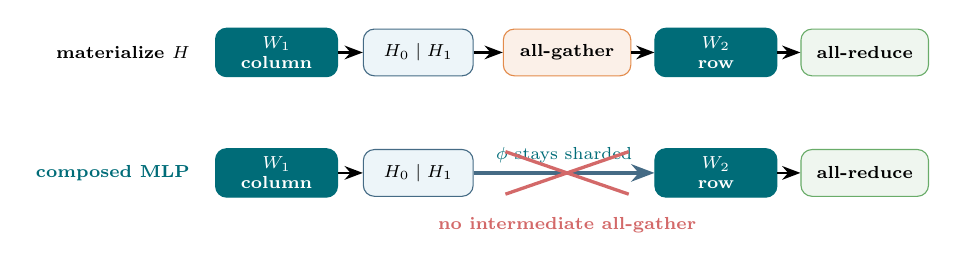
\begin{tikzpicture}[x=1cm,y=1cm,scale=.9,transform shape,every node/.style={font=\scriptsize},
    op/.style={draw=accentdark,fill=accentdark,text=white,rounded corners,minimum width=1.72cm,minimum height=.66cm,align=center,font=\scriptsize\bfseries},
    shard/.style={draw=themebluedraw,fill=themebluebg,rounded corners,minimum width=1.55cm,minimum height=.66cm,align=center},
    collective/.style={draw=successdraw,fill=successbg,rounded corners,minimum width=1.8cm,minimum height=.66cm,align=center,font=\scriptsize\bfseries}]
    \node[anchor=east,font=\scriptsize\bfseries] at (1.45,3.25) {materialize $H$};
    \node[op] (m1) at (2.55,3.25) {$W_1$\\column};
    \node[shard] (mh) at (4.55,3.25) {$H_0\mid H_1$};
    \node[collective,fill=warningbg,draw=warningdraw] (mag) at (6.65,3.25) {all-gather};
    \node[op] (m2) at (8.75,3.25) {$W_2$\\row};
    \node[collective] (mar) at (10.85,3.25) {all-reduce};
    \draw[-{Stealth},thick] (m1)--(mh); \draw[-{Stealth},thick] (mh)--(mag); \draw[-{Stealth},thick] (mag)--(m2); \draw[-{Stealth},thick] (m2)--(mar);
    \node[anchor=east,font=\scriptsize\bfseries,text=accentdark] at (1.45,1.55) {composed MLP};
    \node[op] (c1) at (2.55,1.55) {$W_1$\\column};
    \node[shard] (ch) at (4.55,1.55) {$H_0\mid H_1$};
    \node[op] (c2) at (8.75,1.55) {$W_2$\\row};
    \node[collective] (car) at (10.85,1.55) {all-reduce};
    \draw[-{Stealth},thick] (c1)--(ch);
    \draw[-{Stealth},very thick,themebluedraw] (ch)-- node[above,text=accentdark] {$\phi$ stays sharded} (c2);
    \draw[-{Stealth},thick] (c2)--(car);
    \draw[very thick,alertdraw] (5.78,1.25)--(7.52,1.85);
    \draw[very thick,alertdraw] (5.78,1.85)--(7.52,1.25);
    \node[text=alertdraw,font=\scriptsize\bfseries] at (6.65,.82) {no intermediate all-gather};
  \end{tikzpicture}
  \vspace{4pt}
  \footnotesize $H_i=\phi(XW_{1,i})$, then $Y=\sum_i H_iW_{2,i}$: two GEMMs, one forward collective.
  \smallsource{Hugging Face Ultra-Scale Playbook and Megatron-LM}
\end{frame}

\section{Inside a Transformer block}

\begin{frame}{Attention naturally shards by heads}
  \begin{itemize}
    \setlength{\itemsep}{8pt}
    \item Column-shard the fused $QKV$ projection so each rank owns a subset of heads.
    \item Compute attention locally for those heads.
    \item Row-shard the output projection and all-reduce its partial residual update.
  \end{itemize}
  \begin{alertblock}{Divisibility invariant}
    The number of query heads must divide by tensor-parallel degree. With GQA, key-value head partitioning imposes an additional constraint.
  \end{alertblock}
\end{frame}

\begin{frame}{A layout ledger is the core debugging tool}
  \small
  \begin{tabular}{@{}>{\raggedright\arraybackslash}p{.29\linewidth}>{\raggedright\arraybackslash}p{.31\linewidth}>{\raggedright\arraybackslash}p{.30\linewidth}@{}}
    \toprule
    Point in block & Layout & Local shape \\
    \midrule
    residual input & replicated & $B\times T\times d$ \\
    QKV output & head/feature sharded & $B\times T\times 3d/p$ \\
    local attention output & head sharded & $B\times T\times d/p$ \\
    output projection partial & partial replicated shape & $B\times T\times d$ \\
    after all-reduce & replicated & $B\times T\times d$ \\
    MLP expansion & feature sharded & $B\times T\times 4d/p$ \\
    \bottomrule
  \end{tabular}
  \vfill
  Every operation must declare what is sharded, what is replicated, and what collective changes that layout.
\end{frame}

\begin{frame}{Sequence parallelism removes replicated token activations}
  LayerNorm, dropout, and some elementwise work do not require the full hidden tensor on every rank. Sequence parallelism shards the $B\times T$ token dimension between tensor-parallel regions.
  \begin{columns}[t]
    \begin{column}{0.47\linewidth}
      \begin{block}{Benefit}
        lower activation memory for operations that would otherwise remain replicated
      \end{block}
    \end{column}
    \begin{column}{0.47\linewidth}
      \begin{alertblock}{Cost}
        reduce-scatter and all-gather transitions around tensor-parallel linear regions
      \end{alertblock}
    \end{column}
  \end{columns}
\end{frame}

\begin{frame}{Forward and backward collectives are conjugate}
  \small
  \begin{tabular}{@{}>{\raggedright\arraybackslash}p{.30\linewidth}>{\raggedright\arraybackslash}p{.31\linewidth}>{\raggedright\arraybackslash}p{.29\linewidth}@{}}
    \toprule
    Forward operation & Forward layout change & Backward communication \\
    \midrule
    identity with replicated input & replicated to sharded use & all-reduce input gradient \\
    all-reduce sum & partial to replicated & identity on matching shard flow \\
    reduce-scatter & replicated partials to shard & all-gather \\
    all-gather & shards to replicated & reduce-scatter \\
    \bottomrule
  \end{tabular}
  \vfill
  \begin{alertblock}{Testing rule}
    Compare forward outputs, input gradients, and parameter gradients against an unsharded reference.
  \end{alertblock}
\end{frame}

\checkpoint{layout trace}
  {Trace replicated or sharded status through a column-parallel MLP expansion, activation, row-parallel contraction, and residual add. At which point is communication unavoidable?}

\section{Cost and placement}

\begin{frame}{Communication cost depends on activation size}
  A collective over $B\times T\times d$ elements moves bytes proportional to the activation tensor, not the parameter matrix.
  \[
    S_{\text{act}}=B\,T\,d\,s
  \]
  \begin{itemize}
    \setlength{\itemsep}{7pt}
    \item Larger batch and context increase collective payload.
    \item Higher TP degree shrinks local matmuls and can reduce arithmetic efficiency.
    \item Collective latency and link bandwidth set the exposed cost.
  \end{itemize}
\end{frame}

\begin{frame}{Tensor parallelism belongs on the fastest links}
  \begin{columns}[c]
    \begin{column}{0.48\linewidth}
      \begin{block}{Intra-node}
        High-bandwidth, low-latency GPU fabrics suit frequent activation collectives.
      \end{block}
    \end{column}
    \begin{column}{0.48\linewidth}
      \begin{alertblock}{Across slow links}
        Small per-rank matmuls plus exposed all-reduces can erase the benefit quickly.
      \end{alertblock}
    \end{column}
  \end{columns}
  \vfill
  Keep TP inside a fast island when possible, then use data or pipeline parallelism across nodes.
\end{frame}

\begin{frame}{Choose the smallest degree that solves the constraint}
  \begin{enumerate}
    \setlength{\itemsep}{7pt}
    \item Determine whether a layer's weights or activations fail to fit on one GPU.
    \item Check head, hidden, and MLP divisibility for candidate degrees.
    \item Map the group to the strongest available links.
    \item Measure local matmul efficiency and collective exposure.
    \item Verify numerics against the unsharded block.
  \end{enumerate}
\end{frame}

\checkpoint{degree selection}
  {A model fits with TP=2, but TP=8 gives lower throughput. Explain the result using local matrix shapes, collective frequency, and topology.}

\takeaways
  {Column parallelism shards output features, while row parallelism sums partial outputs.}
  {Their composition keeps intermediate MLP and attention shards local.}
  {A layout ledger and unsharded numerical reference are essential correctness tools.}
  {Tensor parallelism is a fine-grained method that needs large local work and fast links.}
\end{document}
